%% MSR 2027 technical paper — double-anonymous submission format.
%% Deadlines: abstract Mon 20 Oct 2026 AoE, paper Thu 23 Oct 2026 AoE.
%% Limit: 10 pages + 2 pages references. ACM Primary Article Template.
\documentclass[sigconf,review,anonymous]{acmart}

\usepackage{booktabs}
\usepackage{xspace}

%% TODO(camera-ready): set correct rights/DOI info from the ACM eform.
\setcopyright{none}
\acmConference[MSR 2027]{24th International Conference on Mining Software
  Repositories}{April 2027}{Dublin, Ireland}

\newcommand{\structured}{\textsc{structured}\xspace}
\newcommand{\codeonly}{\textsc{code\_only}\xspace}
\newcommand{\rawtext}{\textsc{raw\_text}\xspace}
\newcommand{\rawrerank}{\textsc{raw\_text\_rerank}\xspace}
\newcommand{\oraclecorpus}{\textsc{oracle\_corpus}\xspace}
\newcommand{\oracleself}{\textsc{oracle\_self}\xspace}
\newcommand{\pp}{\,pp}
% Draft-only TODO marker; must be empty before submission.
\newcommand{\todo}[1]{\textcolor{red}{[TODO: #1]}}

\begin{document}

\title[Relevance Without Repair]{Relevance Without Repair: Retrieval Gains Are
  Fragile and Do Not Convert in Synthetic and Algorithmic LLM Program Repair}

%% Anonymous for review (the anonymous option suppresses these).
\author{Anonymous Author(s)}
\affiliation{%
  \institution{Anonymous Institution}
  \city{}
  \country{}}

\begin{abstract}
Retrieval-augmented generation (RAG) is widely assumed to improve LLM-based
automated program repair: retrieve similar past bug fixes, show them to the
model, repair more bugs. We test this assumption with a critical empirical
study built around \emph{structured failure-aware retrieval}, a reranking
method that matches a structured representation of the observed test failure
(failure mode, exception type, suspicious symbols, contract tags) against
repair metadata inferred from each corpus example's fix. Across four benchmarks
(QuixBugs, HumanEvalFix, a contamination-controlled MBPP repair split, and
real repository bugs from PyBugHive), six models, and five retrieval variants,
we find: (1)~structured reranking significantly improves an independent
retrieval-relevance metric on QuixBugs ($p{=}0.0001$) but the gain does not
replicate on a larger benchmark ($n{=}187$, $p{=}0.41$) --- the relevance gain
itself is fragile; (2)~no retrieval variant significantly improves repair over
a no-retrieval baseline anywhere --- downstream effects are
neutral-to-slightly-negative (point estimates $-0.5$ to $-3.7\pp$, equivalent
to baseline within $\pm 10\pp$ but not $\pm 5\pp$); (3)~a planted-corpus
experiment that guarantees a perfect example is present decomposes the failure:
repair then improves by $+14.4$/$+13.4\pp$ ($p{<}0.001$, two models), plain
dense retrieval already surfaces the planted example 100\% of the time, and
structured reranking selects it \emph{less} often (94.1\%). The binding
constraint is primarily \emph{corpus coverage}, not retrieval ranking; ranking
headroom is small and heterogeneous ($+7.5$ to $-1.6\pp$). On real repository
bugs, planting the exact fix converts all four baseline failures
($85.7\%{\to}96.4\%$), directionally supporting coverage transfer.
%% TODO(powered-CI): replace the sentence above with the powered PyBugHive
%% result (116 cases, 10 projects) once the CI experiment lands.
Our results caution that better retrieval relevance is neither robustly
achievable nor sufficient for better repair, and suggest investing retrieval
budgets in corpus coverage and curation rather than reranking sophistication.
\end{abstract}

\begin{CCSXML}
<ccs2012>
<concept>
<concept_id>10011007.10011074.10011099.10011102.10011103</concept_id>
<concept_desc>Software and its engineering~Software testing and debugging</concept_desc>
<concept_significance>500</concept_significance>
</concept>
</ccs2012>
\end{CCSXML}
\ccsdesc[500]{Software and its engineering~Software testing and debugging}

\keywords{automated program repair, retrieval-augmented generation, large
language models, empirical study, negative results}

\maketitle

\section{Introduction}
\label{sec:intro}

Large language models repair a substantial fraction of buggy programs from a
single prompt containing the code and a failing test's output. A natural next
step, borrowed from retrieval-augmented generation (RAG), is to also show the
model \emph{similar past fixes}: retrieve bug-fix pairs from a corpus of
historical repairs, and let the model imitate the relevant repair pattern.
Several recent systems report gains from exactly this recipe
\cite{recode,inferfix,rapgen,ragfix}, and the intuition is compelling ---
if a developer benefits from seeing how a similar bug was fixed before, an LLM
should too.

This paper reports a critical empirical study of that intuition. We built the
strongest retrieval signal we could construct for the repair setting:
\emph{structured failure-aware retrieval}, which parses the observed test
failure into a structured state (failure mode, exception type, failing test
name, assertion summary, suspicious symbols, contract tags) and reranks
dense-retrieved candidates by compatibility between that state and repair
metadata inferred from each corpus example's diff
(Section~\ref{sec:method}). We then asked three increasingly uncomfortable
questions:

\begin{description}
  \item[RQ1 (Relevance)] Does structured failure-aware reranking retrieve
    more fix-relevant examples than dense code retrieval?
  \item[RQ2 (Conversion)] Do more relevant examples produce more successful
    repairs?
  \item[RQ3 (Mechanism)] When retrieval fails to help, what is the binding
    constraint --- the ranking of the corpus, or the corpus itself?
  \item[RQ4 (Transfer)] Does the answer transfer from synthetic benchmark
    bugs to real repository bugs?
\end{description}

\noindent
Our answers, established across four benchmarks (QuixBugs, HumanEvalFix, a
contamination-controlled MBPP repair split, and real repository bugs from
PyBugHive), six models (GPT-4o, GPT-4.1, GPT-4o-mini, Llama-3-8B,
Llama-3.3-70B, Qwen2.5-7B), and five retrieval variants, are largely
negative --- and, we argue, more useful than another reported win:

\textbf{The relevance gain is real but fragile (RQ1).} Structured reranking
significantly improves an independent, vocabulary-free relevance metric on
QuixBugs ($+13\%$, Wilcoxon $p{=}0.0001$, $n{=}40$), but the gain does
\emph{not} replicate on a larger benchmark (MBPP-holdout, $n{=}187$: $-0.008$,
$p{=}0.41$). A skeptic may reasonably treat the larger-sample null as the
better estimate.

\textbf{Relevance does not convert (RQ2).} Across all models, corpora, and
benchmarks, no retrieval variant significantly beats the no-retrieval
baseline; every point estimate is neutral-to-slightly-negative ($-0.5$ to
$-3.7\pp$). Equivalence testing bounds any undetected effect: results are
equivalent to baseline within $\pm 10\pp$ (though not within the stricter
$\pm 5\pp$), with minimum detectable effects of $4.8$--$9.1\pp$.

\textbf{The binding constraint is corpus coverage, not ranking (RQ3).} A
planted-corpus experiment guarantees that a \emph{perfect} example (the test
problem's own buggy$\to$fixed pair) is present in the corpus. Repair then
jumps by $+21.9\pp$ ($p{<}0.0001$) --- and plain dense retrieval already
surfaces the planted example 100\% of the time, while structured reranking
selects it \emph{less} often (94.1\%). Decomposing the gap between baseline,
the best \emph{real} corpus example (\oraclecorpus), and the planted perfect
example shows coverage headroom of $+14.4$/$+13.4\pp$ (significant, two
models) against ranking headroom of $+7.5$/$-1.6\pp$ (marginal to negative).
When a sufficiently relevant example exists, dense retrieval finds it; when
none exists --- the common case on realistic corpora --- no reranker can help.

\textbf{Real-bug transfer is directionally supported (RQ4).} On real
repository bugs (PyBugHive \texttt{black}), planting the exact fix converted
all four baseline failures ($85.7\%{\to}96.4\%$), with the repair applied
through a line-range patch layer on large files. This result is underpowered
(McNemar $p{=}0.375$);
%% TODO(powered-CI): replace with the powered 116-case, 10-project result and
%% its McNemar p once the CI experiment completes; rewrite this paragraph as a
%% headline finding if significant.
a powered replication across 10 projects is in progress.

\smallskip
\noindent\textbf{Contributions.}
\begin{itemize}
  \item A structured failure-aware retrieval method for program repair with an
    explicit, ablatable reranking function over six failure-state fields
    (each of five fields contributes measurably on QuixBugs).
  \item A statistically grounded negative result: retrieval-augmented repair
    is neutral-to-slightly-negative for capable models on synthetic and
    algorithmic benchmarks, with equivalence bounds and minimum detectable
    effects reported rather than bare non-significance.
  \item A planted-corpus decomposition isolating corpus coverage from
    retrieval ranking, replicated across two model families, that locates the
    binding constraint in coverage and shows reranking sophistication is
    downstream-inert.
  \item A cost analysis showing structured RAG is Pareto-dominated by the
    baseline for repair ($\sim$4$\times$ prompt tokens for zero-to-negative
    accuracy return), and actionable guidance: invest in corpus coverage, not
    reranking.
\end{itemize}

\section{Background and Related Work}
\label{sec:related}

\paragraph{LLM-based program repair.} Modern repair pipelines prompt an LLM
with buggy code and, usually, an observed failure (test output, stack trace),
and validate candidate patches against the test suite. Benchmarks span
algorithmic bugs (QuixBugs~\cite{quixbugs}), function-level edits
(HumanEvalFix~\cite{octopack}), synthetic mutations
(MBPP-derived~\cite{mbpp}), and real repository bugs
(BugsInPy~\cite{bugsinpy}, PyBugHive~\cite{pybughive}). Our study uses all
four regimes deliberately: the first three give executable, well-powered
comparisons; the last tests external validity.

\paragraph{Retrieval-augmented repair.} Several systems retrieve historical
bug-fix examples to condition repair. InferFix~\cite{inferfix} retrieves by
static-analyzer bug type; ReCode~\cite{recode} retrieves by algorithm type;
RAP-Gen~\cite{rapgen} learns a hybrid retriever over CodeT5. Our retrieval
signal differs: we extract a structured state from the \emph{dynamic} test
failure (runtime signal), which is orthogonal to static bug types, and we make
the reranking function explicit and ablatable rather than learned
end-to-end. Direct numeric comparison with these systems is infeasible
(closed source, different languages); our contribution is not a better
system but a controlled analysis of whether the retrieval component can pay
off at all.

RAGFix~\cite{ragfix} retrieves Stack Overflow posts through a
question-answering knowledge graph and reports repair gains on HumanEvalFix
with Llama-3 models --- a different knowledge source (crowd discussion rather
than bug-fix pairs), but the same underlying bet that retrieved context
improves repair. In a recomputation from its released per-example outputs,
the reported 70B improvement is consistent with a post-processing
(import-fixing) artifact rather than retrieval itself; a controlled ablation
on identical outputs would be needed to confirm this, so we flag it as a
caveat rather than a claim. Our own de-confounded measurements
(Section~\ref{sec:results-conversion}) agree with the direction that
retrieval is neutral-to-harmful for capable models on this benchmark.

\paragraph{Negative and analytical results on RAG.} Outside repair, RAG
studies increasingly report conditions under which retrieval does not help or
hurts: irrelevant retrieved context measurably degrades LLM
reasoning~\cite{distracted}, models underuse information positioned
mid-context~\cite{lostinmiddle}, and retrieval helps mainly where the
model's parametric knowledge is weak~\cite{whennottotrust} --- a pattern our
headroom results echo in the repair setting
(Section~\ref{sec:results-mechanism}). Our planted-corpus design contributes
a repair-specific mechanism: it separates \emph{whether the corpus contains a
sufficiently relevant example} (coverage) from \emph{whether the retriever
surfaces it} (ranking), which prior repair evaluations conflate.

\section{Structured Failure-Aware Retrieval}
\label{sec:method}

\subsection{Pipeline}
Our repair pipeline takes buggy Python code plus a raw failure signal
(pytest output) and proceeds in five steps: (1)~extract a \emph{structured
failure state} from the failure signal; (2)~dense-retrieve candidate bug-fix
pairs from a FAISS index of corpus examples embedded with
all-MiniLM-L6-v2~\cite{sbert} over the buggy code; (3)~rerank the candidate
pool with one of the variants below; (4)~prompt the LLM with the bug, the
failure signal, and the top-$k$ ($k{=}2$) retrieved examples rendered as
compact buggy$\to$fixed diffs plus an inferred one-line ``repair lesson'';
(5)~apply the edit and run the tests. Small files are replaced whole; large
files (${>}40$k characters) are edited through a strict JSON line-range patch
schema with validation retry, which matters for repository-scale bugs
(Section~\ref{sec:results-transfer}).

\subsection{Failure state and repair metadata}
The query-side \emph{failure state} has six fields extracted from the failure
signal: \texttt{failure\_mode}, \texttt{exception\_type},
\texttt{test\_name}, \texttt{assertion\_summary},
\texttt{suspicious\_symbols}, and \texttt{contract\_tags}. On the corpus
side, each example's buggy$\to$fixed diff is mined for \emph{repair
metadata}: \texttt{repair\_pattern\_tags}, \texttt{suspicious\_symbols},
\texttt{changed\_operators}, \texttt{edit\_scope}, \texttt{file\_family}, and
\texttt{changed\_lines}.

\subsection{Retrieval variants}
We compare five variants: \textsc{baseline} (no retrieval); \codeonly (dense
retrieval on buggy code, rank = dense rank); \rawtext (dense retrieval on
buggy code + raw failure text); \rawrerank (dense retrieval + lexical
failure-text reranking); and \structured, our method, which scores each
candidate at dense rank $r$ as
\begin{align*}
\mathit{score} ={}& 1.0\cdot\mathit{dense}(r)
  + 0.8\cdot\mathit{tagOverlap}
  + 0.7\cdot\mathit{symOverlap} \\
  &+ 0.8\cdot\mathit{modeCompat}
  + 0.5\cdot\mathit{excCompat}
  + 0.2\cdot\mathit{fileFam} \\
  &- \mathit{changedLines}/400 .
\end{align*}
Overlaps are Jaccard similarities between failure-state fields and repair
metadata; compatibility terms encode hand-written failure-mode and
exception-class compatibility. The weights were fixed once, early, on
QuixBugs traces, and never tuned against any downstream result reported here.

A per-field ablation on QuixBugs (GPT-4o) confirms the signal is not
redundant: removing any one of \texttt{contract\_tags},
\texttt{suspicious\_symbols}, \texttt{failure\_mode}, \texttt{test\_name}, or
\texttt{assertion\_summary} costs one repaired problem (37/40${\to}$36/40);
only \texttt{exception\_type} contributes nothing on this benchmark.

\section{Study Design}
\label{sec:design}

\subsection{Benchmarks}
\textbf{QuixBugs}~\cite{quixbugs}: 40 algorithmic Python bugs; controlled
setting. \textbf{HumanEvalFix}~\cite{octopack}: 164 function-level tasks;
robustness setting. \textbf{MBPP-holdout}: a contamination-controlled repair
split we construct from MBPP~\cite{mbpp}: 187 test problems with synthetic
single-operator mutations, and a 508-pair retrieval corpus whose problems are
disjoint from the test set (zero overlap). \textbf{PyBugHive}
\texttt{black}~\cite{pybughive}: 34 real repository bugs with issue-linked
fixed commits, evaluated end-to-end (checkout, environment build, patch, test
run).
%% TODO(powered-CI): extend to the 116-case, 10-project powered setting.

\subsection{Retrieval corpora}
The primary corpus is 551 real-world bug-fix pairs from
BugsInPy~\cite{bugsinpy}. For PyBugHive we use a project-held-out variant
(277 pairs, all 11 PyBugHive projects removed) to control contamination ---
without this control, same-project corpus entries inflate apparent RAG effects.
For MBPP we additionally build a genuine MBPP corpus (1{,}041 pairs) to test
corpus--benchmark domain match. Planted-corpus variants
(Section~\ref{sec:results-mechanism}) add each test problem's exact
buggy$\to$fixed pair.

\subsection{Models}
GPT-4o, GPT-4.1, and GPT-4o-mini (OpenAI); Llama-3-8B-Instruct,
Llama-3.3-70B-Instruct-Turbo, and Qwen2.5-7B-Instruct-Turbo (Together~AI).
All runs use temperature~0, a single attempt, and a single candidate patch
unless stated otherwise. Temperature-0 reruns flip at most 1/187 outcomes, so
single-trial results are representative; where variance matters (QuixBugs) we
report 5-trial means.

\subsection{Measures and statistics}
\textbf{Retrieval relevance} is measured two ways: a repair-pattern
\emph{tag-compatibility} proxy (top-5 Jaccard against ground-truth fix tags),
and an \emph{independent, vocabulary-free} metric --- the cosine similarity
between a candidate example's fix diff and the ground-truth fix diff ---
which shares no vocabulary with the reranker objective and thus defuses
circularity. We report the tag proxy only alongside the independent metric,
because it overstates ($+81\%$ vs $+13\%$ on QuixBugs).
%% TODO(audit): add blind two-annotator human relevance audit (Cohen's kappa)
%% here and in RQ1 results once annotation completes.
\textbf{Repair success} is test-suite pass after applying the candidate
patch. \textbf{Significance}: exact McNemar tests on paired outcomes for all
downstream comparisons; Wilcoxon signed-rank plus bootstrap CIs for
relevance. \textbf{Equivalence}: TOST at $\pm 5\pp$ and $\pm 10\pp$ margins
with minimum detectable effects (MDE) at 80\% power, so that
non-significance is never silently read as ``no effect.''

\section{Results}
\label{sec:results}

\subsection{RQ1: Relevance --- improved, but fragile}
\label{sec:results-relevance}

On QuixBugs ($n{=}40$), \structured improves the independent fix-diff
relevance metric over \codeonly at every depth (top-5: $0.234$ vs $0.207$;
mean difference $+0.027$, 95\%~CI $[+0.016,+0.037]$; Wilcoxon $p{=}0.0001$;
higher on 31/40 problems). The tag-compatibility proxy shows the same
direction but overstates it ($0.394$ vs $0.218$, $+81\%$, against $+13\%$ on
the independent metric); we therefore treat the tag proxy as illustrative
only.

However, the gain \emph{does not replicate} on MBPP-holdout ($n{=}187$):
\codeonly $0.464$ vs \structured $0.456$ (mean difference $-0.008$, 95\%~CI
$[-0.025,+0.009]$, $p{=}0.41$). Two interpretations are compatible with one
positive and one null: (a)~the gain is benchmark-specific --- MBPP's
single-operator mutations leave a thin failure signal, and dense retrieval
already matches the near-identical buggy code, leaving no room for failure
structure to help; or (b)~the gain is simply not robust, and the
larger-sample null is the better estimate. We cannot distinguish these from
the available data, and interpretation~(a) was constructed post hoc. Either
way, the one clean positive in this study is fragile --- which sharpens
rather than weakens the questions that follow.
%% TODO(audit): report the blind human relevance audit (two annotators,
%% Cohen's kappa, per-variant human relevance rates) as the third measure.

\begin{table}
\caption{Independent relevance metric (cosine of candidate fix diff to
ground-truth fix diff), top-5 mean.}
\label{tab:relevance}
\begin{tabular}{lrrr}
\toprule
Benchmark & \codeonly & \structured & $p$ \\
\midrule
QuixBugs ($n{=}40$) & 0.207 & \textbf{0.234} & 0.0001 \\
MBPP-holdout ($n{=}187$) & 0.464 & 0.456 & 0.41 (ns) \\
\bottomrule
\end{tabular}
\end{table}

\subsection{RQ2: Conversion --- neutral to slightly negative}
\label{sec:results-conversion}

\begin{table}
\caption{Downstream repair vs.\ no-retrieval baseline (single attempt,
$k{=}2$). All differences non-significant by exact McNemar.}
\label{tab:downstream}
\begin{tabular}{llrrr}
\toprule
Benchmark & Model & base & \structured & $p$ \\
\midrule
QuixBugs & GPT-4o & 35/40 & 37/40 & ns \\
QuixBugs & GPT-4.1 & 36/40 & 35/40 & ns \\
QuixBugs & GPT-4o-mini & 33/40 & 30/40 & ns \\
HumanEvalFix & GPT-4o & 80.5\% & 76.8\% & 0.109 \\
HumanEvalFix & GPT-4.1 & 79.9\% & 78.7\% & 0.727 \\
HumanEvalFix & GPT-4o-mini & 68.3\% & 66.5\% & 0.629 \\
HumanEvalFix & Llama-3.3-70B & 69.5\% & 67.7\% & 0.648 \\
MBPP-holdout & GPT-4o-mini & 93.0\% & 91.4\% & 0.55 \\
MBPP-holdout & Llama-3-8B & 64.7\% & 64.2\% & 1.0 \\
\bottomrule
\end{tabular}
\end{table}

Table~\ref{tab:downstream} summarizes downstream repair. No comparison is
significant, and the pattern is consistent: \structured never beats the
baseline, and every HumanEvalFix and MBPP point estimate is negative
($-0.5$ to $-3.7\pp$). The QuixBugs GPT-4o ``$+2$'' is within run-to-run
variance (5-trial means: baseline $89.5\%$, \structured $91.0\%$,
overlapping). \codeonly and the raw-text variants behave like \structured\
throughout (omitted rows differ by at most one problem).

Because ``not significant'' is not ``no effect,'' we also report equivalence:
TOST finds all comparisons equivalent to baseline within $\pm 10\pp$ but not
within $\pm 5\pp$; minimum detectable effects range $4.8$--$9.1\pp$. For the
most capable model (GPT-4o on HumanEvalFix, $-3.7\pp$), the Wald 90\%~CI
$[-6.8,-0.5]$ excludes zero while the exact McNemar $p{=}0.109$ does not; the
discordant count is small ($b{=}8$, $c{=}2$), where the normal approximation
is unreliable, so we defer to the exact test and read the result as
\emph{borderline small harm}. The honest summary of RQ2 is
\textbf{neutral-to-slightly-negative}, bounded by $\pm 10\pp$ --- not clean
neutrality.

Two further controls rule out easy explanations. \emph{Corpus--benchmark
domain match} is not the lever: swapping the BugsInPy corpus for a genuine
MBPP corpus on HumanEvalFix moves results by small, inconsistent,
non-significant amounts (GPT-4o $-3.7{\to}-2.5$; Llama-70B $-1.8{\to}-6.7$).
\emph{Weak-model formatting} is a confound to remove, not a RAG win in
disguise: Llama-3-8B initially collapsed under the longer RAG prompt (123/164
syntax-invalid outputs); with robust extraction the collapse disappears
(0/187) and retrieval remains neutral ($64.7\%$ vs $64.2\%$).

\subsection{RQ3: Mechanism --- coverage dominates ranking}
\label{sec:results-mechanism}

If retrieval cannot help, is that because the corpus lacks relevant examples
(coverage), or because the retriever fails to surface them (ranking)? We
answer with two forcing experiments on MBPP-holdout.

\textbf{\oraclecorpus} bypasses retrieval entirely and shows the model the
\emph{best real} example in the (disjoint) corpus, selected by ground-truth
fix similarity: the ceiling attributable to perfect \emph{ranking}.
\textbf{Planted corpus} instead guarantees \emph{coverage}: each test
problem's exact buggy$\to$fixed pair is inserted into the corpus, and normal
retrieval runs.

\begin{figure}
\centering
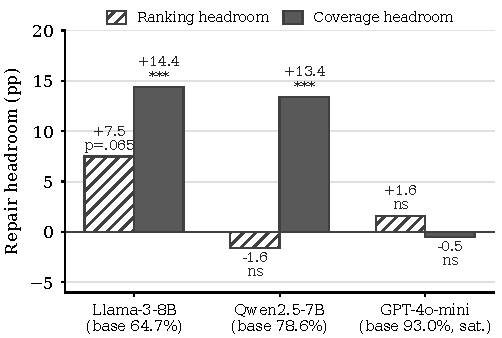
\includegraphics{figures/decomposition.pdf}
\caption{The decomposition of Table~\ref{tab:decomposition}: coverage
headroom (guaranteeing a perfect example exists) dwarfs ranking headroom
(perfectly selecting the best real example) on both non-saturated models and
vanishes on the saturated control. $^{***}$: $p{<}0.001$, exact McNemar.}
\label{fig:decomposition}
\end{figure}

\begin{table}
\caption{Coverage-vs-ranking decomposition ($n{=}187$; exact McNemar vs
baseline). Ranking headroom = \oraclecorpus $-$ base; coverage headroom =
planted $-$ \oraclecorpus.}
\label{tab:decomposition}
\begin{tabular}{lrrrr}
\toprule
Model (base) & \oraclecorpus & planted & rank.\ hr & cov.\ hr \\
\midrule
Llama-3-8B (64.7\%) & 72.2\% & 86.6\% & $+7.5$\rlap{$^{p=.065}$} & $\mathbf{+14.4}$\rlap{$^{***}$} \\
Qwen2.5-7B (78.6\%) & 77.0\% & 90.4\% & $-1.6$\rlap{$^{ns}$} & $\mathbf{+13.4}$\rlap{$^{***}$} \\
GPT-4o-mini (93.0\%) & 94.7\% & 94.1\% & $+1.6$\rlap{$^{ns}$} & $-0.5$\rlap{$^{ns}$} \\
\bottomrule
\end{tabular}
\end{table}

Table~\ref{tab:decomposition} and Figure~\ref{fig:decomposition} give the
central result. With a perfect example guaranteed present, repair jumps $+21.9\pp$ over baseline for
Llama-3-8B ($64.7\%{\to}86.6\%$, $p{<}0.0001$) and $+11.8\pp$ for Qwen2.5-7B
--- so retrieved examples \emph{can} convert failures when a sufficiently
relevant one exists. Decomposing that gain: \textbf{coverage headroom is
large and significant on both non-saturated models} ($+14.4$ and $+13.4\pp$)
and zero on the saturated control, while \textbf{ranking headroom is small
and heterogeneous} ($+7.5\pp$ marginal on Llama; $-1.6\pp$ on Qwen, where
even forcing the best real example does not help). We refuse to average the
two into a single ``ranking gap'': the honest claim is that the binding
constraint is \emph{primarily corpus coverage}, with inconsistent, at-best
marginal ranking headroom.

The most damaging finding for reranking sophistication: when the perfect
example is present, \emph{plain dense retrieval surfaces it in the top-$k$
100\% of the time}, while \structured reranking demotes it out of the top-$k$
in 11/187 cases (94.1\%) --- and repair conversion is identical for both
($86.6\%$). The relevance-proxy improvement of RQ1, even where it holds,
does not translate into better best-example selection; it slightly degrades
it. Relevance-to-repair conversion also fails at the instance level: among
the 37 problems where retrieval flips the 8B outcome (18 wins, 19 losses),
the mean retrieved-example relevance of wins ($2.645$) is indistinguishable
from losses ($2.621$).

For completeness, \oracleself\ (showing the model its own problem's exact
fix pattern) reaches $90.4\%$ ($+25.7\pp$, $p{<}0.0001$) on 8B --- a sanity
check that the model can exploit a near-identical example, not a deployable
ceiling.

\subsection{RQ4: Transfer to real repository bugs}
\label{sec:results-transfer}

Synthetic mutations make ``perfect examples'' constructible by design, so RQ3
could in principle be an artifact of the synthetic regime. We test transfer
on real PyBugHive \texttt{black} bugs end-to-end (environment build, patch
application through the line-range layer, full test suite).

With the project-held-out corpus (contamination-controlled), baseline,
\codeonly, and \structured all repair 23/34 --- retrieval is exactly neutral
on real bugs, consistent with RQ2. Planting the exact buggy$\to$fixed file
pairs into the corpus (34 plants + 551 filler) lifts GPT-4o-mini from
$85.7\%$ to $96.4\%$ on the 28 cleanly-paired cases, converting \emph{all
four} baseline failures while regressing one (McNemar $b{=}1$, $c{=}4$,
$p{=}0.375$). The patch layer did apply the planted fixes on large formatter
files, so the coverage effect is not blocked by repository-scale mechanics.

This transfer result is directionally positive but underpowered: black's high
baseline leaves only four failures to convert.
%% TODO(powered-CI): replace this paragraph with the powered result over 116
%% cases / 10 projects (pandas, jax, freqtrade, salt, spaCy, poetry, ...)
%% from the CI experiment; report pooled exact McNemar and per-project
%% breakdown, and update the abstract and Section 1 accordingly.
A powered replication over all 116 supported PyBugHive cases across 10
projects (executing in x86 containers to lift the local environment ceiling)
is in progress; we will report it in the final version.

\section{Discussion}
\label{sec:discussion}

\paragraph{Why doesn't relevance convert?} Our decomposition suggests a
simple economy: a retrieved example helps only if it is \emph{sufficiently}
relevant to the specific fix, and realistic corpora rarely contain such an
example for a given new bug. When one exists (planted), even plain dense
retrieval finds it and repair converts; when none exists, improving the
\emph{ordering} of insufficient examples cannot manufacture the missing
knowledge. Reranking sophistication addresses the part of the problem that
was not binding.

\paragraph{Headroom scales with what the model currently fails.} The planted
gain is $+14$/$+13\pp$ on the two models with mid-range base accuracy and
$\sim 0$ on the saturated one. We frame this as ``headroom scales with the
fraction of currently-failed problems that a perfect example would fix''
rather than a categorical knowledge-gap principle: Qwen2.5-7B ($78.6\%$ base)
is close to GPT-4o's HumanEvalFix base ($80.5\%$), and the distinguishing
variable in our data is base accuracy, not model family.

\paragraph{Cost: structured RAG is Pareto-dominated for repair.} Measured on
HumanEvalFix GPT-4o traces, the structured prompt averages 4{,}632 input
characters ($\approx$1{,}158 tokens) against 1{,}199 ($\approx$300) for the
baseline --- a ${\sim}4\times$ input multiplier, plus embedding, indexing,
and retrieval infrastructure --- for equal-or-worse accuracy. In absolute
terms the marginal cost is small ($\sim$\$0.002/repair at GPT-4o input
pricing); the point is direction: you pay more and get nothing. The
actionable guidance for practitioners follows from RQ3: \textbf{spend the
retrieval budget on corpus coverage and curation, not reranking
sophistication} --- the two are separable, and only one showed positive
returns anywhere in this study.

\paragraph{Implications for reported RAG-repair gains.} Contamination and
post-processing can masquerade as retrieval effects. In our own PyBugHive
setting, an uncontrolled corpus (containing same-project entries) flipped
results from neutral to strongly negative-looking for RAG variants; the
project-held-out control removed the artifact. Externally, our recomputation
of RAGFix's released outputs (Section~\ref{sec:related}) is consistent with a
post-processing artifact. We recommend that RAG-repair evaluations
(i)~hold out same-project corpus entries, (ii)~ablate post-processing
separately from retrieval, and (iii)~report equivalence bounds, not bare
non-significance.

\section{Threats to Validity}
\label{sec:threats}

\paragraph{External validity.} Our \emph{powered} executable results are on
algorithmic and synthetic-mutation benchmarks (QuixBugs, HumanEvalFix, MBPP
mutations). The real-repository evidence (PyBugHive \texttt{black}) is
directionally consistent but underpowered ($p{=}0.375$).
%% TODO(powered-CI): update once the 116-case experiment lands.
Relatedly, the coverage thesis relies on a ``perfect example'' being
\emph{constructible}, which is cleanest for synthetic mutations; on real bugs
the notion is fuzzier. The black experiment partially addresses this ---
planting exact pairs did convert real baseline failures through the patch
layer --- but a powered real-bug decomposition remains the largest open
threat.

\paragraph{Construct validity.} Both automated relevance measures are
proxies. The tag-compatibility metric shares vocabulary with the reranker and
overstates; we therefore lead with the independent fix-diff metric, which
shares nothing with the reranker objective. A blind two-annotator human audit
is the missing gold standard.
%% TODO(audit): replace with audit results (rates + Cohen's kappa) when done.
The QuixBugs relevance gain, our one clean positive, does not replicate on
MBPP; we present both the benchmark-specificity and the not-robust
interpretations rather than asserting either.

\paragraph{Internal validity.} The coverage-vs-ranking decomposition is
shown on one bug family (MBPP mutations) with two non-saturated models plus a
saturated control; the direction replicates across two independent
architectures, but the magnitudes are benchmark-specific. \oracleself\ is a
sanity check, not a headroom estimate, and no claim rests on it. Temperature-0
runs are near-deterministic (at most 1/187 flips), so single-trial deltas are
not noise artifacts; QuixBugs results are additionally reported as 5-trial
means.

\paragraph{Statistical power.} With $n{=}40$--$187$, minimum detectable
effects are $4.8$--$9.1\pp$; effects smaller than that cannot be excluded,
and our equivalence claims are correspondingly bounded at $\pm 10\pp$ (weak
equivalence). We report exact tests throughout and defer to them where
approximations disagree.

\paragraph{RAGFix recomputation.} Our recomputation uses RAGFix's released
per-example outputs but compares \emph{different runs}; it is inferential,
not a controlled post-processing ablation, and we accordingly claim only
consistency with an artifact, not proof.

\section{Conclusion}
\label{sec:conclusion}

We set out to make retrieval-augmented program repair work better by making
retrieval more relevant, and instead produced a cautionary decomposition of
why that framing fails. Structured failure-aware reranking can improve a
retrieval-relevance proxy, but the gain is fragile across benchmarks, and
even where it holds it does not convert to repair: downstream effects are
neutral-to-slightly-negative across six models and four benchmarks, bounded
within $\pm 10\pp$. A planted-corpus experiment locates the binding
constraint: when a sufficiently relevant example exists in the corpus, plain
dense retrieval already surfaces it and repair improves by double digits;
when it does not --- the common case --- no amount of reranking
sophistication helps, and our reranker even selects the perfect example
slightly less often than dense retrieval. Coverage dominates ranking. On real
repository bugs the same pattern holds directionally, with a powered
replication in progress.

For practitioners, the guidance is concrete: before investing in retrieval
scoring for repair, invest in the corpus --- coverage and curation are where
the recoverable headroom sits, and the headroom scales with how much the
model currently fails. For evaluators, our results argue for
contamination-controlled corpora, post-processing ablations, and equivalence
bounds as defaults in RAG-repair studies. All artifacts, including the
planted-corpus builders and the CI harness for powered real-bug replication,
are released for reuse.


\section*{Data Availability}
%% The anonymized package is built by scripts/make_anonymized_archive.sh
%% (dist/replication_anonymized.zip, verified free of identifying strings).
%% TODO(submission): upload that zip to Zenodo (anonymized record) at
%% submission time and paste the DOI here; MSR's open-science policy requires
%% an archival host (Zenodo/Software Heritage), not GitHub alone, under an
%% open license (CC0/CC-BY 4.0).
All code, corpora-construction scripts, per-case results, significance and
equivalence analyses, the blind-audit tooling, and the CI workflow for the
repository-bug experiment are available in our anonymized replication
package: \todo{Zenodo DOI of the prepared archive}.

\bibliographystyle{ACM-Reference-Format}
\bibliography{references}

\end{document}
